\documentclass[border=5mm]{standalone}
\usepackage{xcolor}
\usepackage{tikz}
\usetikzlibrary{positioning}
\usetikzlibrary{calc}
\begin{document}

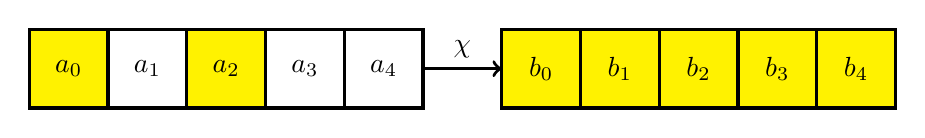
\begin{tikzpicture}
    [%%%%%%%%%%%%%%%%%%%%%%%%%%%%%%
        box/.style={rectangle,draw=black,very thick, minimum size=1cm}
    ]%%%%%%%%%%%%%%%%%%%%%%%%%%%%%%
\definecolor{darkgreen}{rgb}{0.0, 0.7, 0.5}
\foreach \x in {0,1,...,4}{
    \node[box] at (\x,0){$a_\x$};
}

\node[box,fill=yellow] at (0,0){$a_0$};
\node[box,fill=yellow] at (2,0){$a_2$};

\node[box,fill=yellow] at (6,0){$b_0$};
\node[box,fill=yellow] at (7,0){$b_1$};
\node[box,fill=yellow] at (8,0){$b_2$};
\node[box,fill=yellow] at (9,0){$b_3$};
\node[box,fill=yellow] at (10,0){$b_4$};

\draw [->,very thick] (4.5,0) -- node [above] {$\chi$} (5.5,0);

\end{tikzpicture}
\end{document}